
\begin{table}[H]
\centering
\begin{tabular}{lllllll}
\textbf{Rows} & \textbf{1} & \textbf{10} & \textbf{100} & \textbf{1000} & \textbf{10000} & \textbf{100000} \\
\textbf{Get reservations} & 1931.07 & 1638.79 & 1644.44 & 1643.86 & 1644.2 & 1646.79\\
\textbf{Create reservation} & 449.72 & 454.17 & 455.67 & 447.36 & 381.91 & 131.17\\
\textbf{Update reservation} & 1769.77 & 1780.6 & 1780.72 & 1784.31 & 1786.11 & 1777.35\\
\textbf{Delete reservation} & 2901.17 & 2881.88 & 2895.9 & 2890.51 & 2891.5 & 2891.63
\end{tabular}
\caption{Througput in requests per second for server-side operations per number of rows client may access for the REST server.}
\label{tab:server-rest-experiment}
\end{table}

\begin{table}[H]
\centering
\begin{adjustbox}{width=\textwidth}
\begin{tabular}{lllllll}
\textbf{Rows} & \textbf{1} & \textbf{10} & \textbf{100} & \textbf{1000} & \textbf{10000} & \textbf{100000} \\
\textbf{Get reservations} & 51.68 (55.11) & 60.9 (62.69) & 60.7 (62.22) & 60.72 (62.38) & 60.7 (62.29) & 60.61 (62.73)\\
\textbf{Create reservation} & 220.97 (307.43) & 218.93 (310.32) & 218.16 (311.85) & 222.24 (315.77) & 260.36 (343.12) & 756.63 (816.46)\\
\textbf{Update reservation} & 56.35 (60.04) & 56.01 (59.21) & 56.01 (59.58) & 55.89 (59.18) & 55.84 (59.7) & 56.11 (59.5)\\
\textbf{Delete reservation} & 34.34 (42.28) & 34.58 (42.49) & 34.4 (42.76) & 34.48 (42.87) & 34.46 (43.2) & 34.45 (42.81)
\end{tabular}
\end{adjustbox}
\caption{Average latency in milliseconds for server-side operations per number of rows client may access for the REST server. The 95th percentile of latency is shown in parentheses.}
\label{tab:server-rest-experiment-latency}
\end{table}

\begin{figure}[H]
    \centering

\begin{subfigure}[b]{0.48\textwidth}
    \centering
    
\resizebox{\textwidth}{!}{
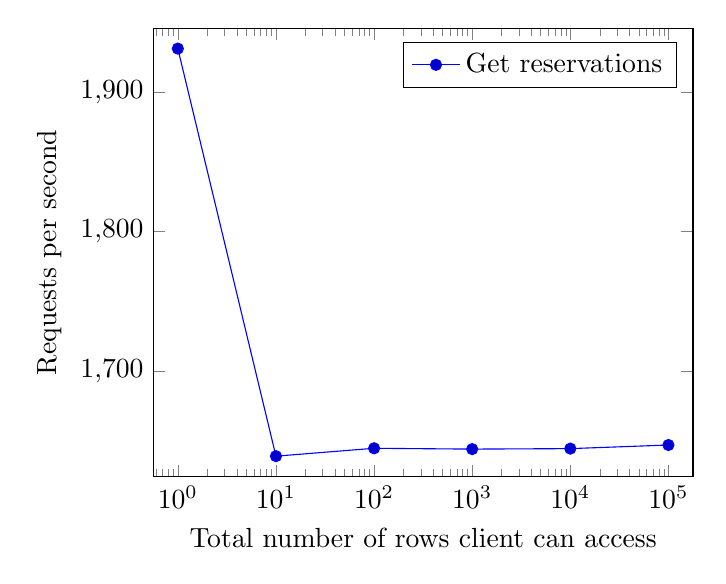
\begin{tikzpicture}
\begin{axis}[
    scaled x ticks=false,
    xticklabel style={
        /pgf/number format/fixed,
    },
    enlargelimits=0.05,
    xmode=log,
    legend pos=north east,
	ylabel=Requests per second,
    xlabel=Total number of rows client can access,
]
\addplot coordinates {
(1,1931.072897046547)
(10,1638.7945274299673)
(100,1644.4413544126533)
(1000,1643.8580304271343)
(10000,1644.203858168117)
(100000,1646.7911417681348)
};
\legend{Get reservations}
\end{axis}
\end{tikzpicture}

}

    \caption{Throughput in requests per second for getting reservations.}
    \label{fig:server-rest-get}
\end{subfigure}
\hfill
\begin{subfigure}[b]{0.48\textwidth}
    \centering
    
\resizebox{\textwidth}{!}{
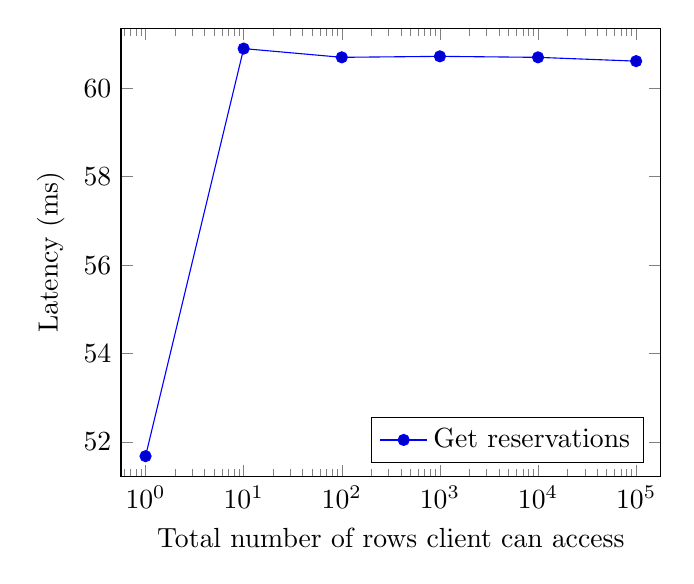
\begin{tikzpicture}
\begin{axis}[
    scaled x ticks=false,
    xticklabel style={
        /pgf/number format/fixed,
    },
    enlargelimits=0.05,
    xmode=log,
    legend pos=south east,
	ylabel=Latency (ms),
    xlabel=Total number of rows client can access,
]
\addplot coordinates {
(1,51.67746153200047)
(10,60.89765806341677)
(100,60.700292285733276)
(1000,60.72230031960203)
(10000,60.69969373819569)
(100000,60.61427298150261)
};
\legend{Get reservations}
\end{axis}
\end{tikzpicture}

}

    \caption{Average latency in milliseconds for getting reservations.}
    \label{fig:server-rest-get-latency}
\end{subfigure}
\\
\begin{subfigure}[b]{0.48\textwidth}
    \centering
    
\resizebox{\textwidth}{!}{
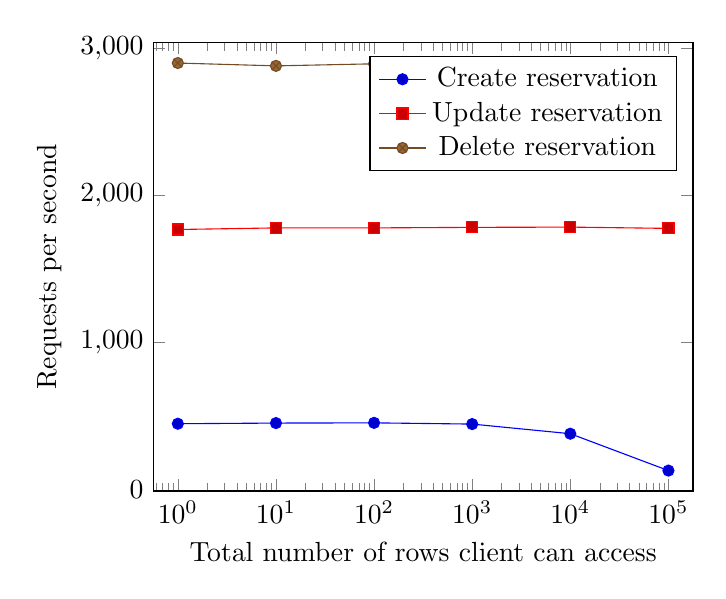
\begin{tikzpicture}
\begin{axis}[
    scaled x ticks=false,
    xticklabel style={
        /pgf/number format/fixed,
    },
    enlargelimits=0.05,
    xmode=log,
    legend pos=north east,
	ylabel=Requests per second,
    xlabel=Total number of rows client can access,
]
\addplot coordinates {
(1,449.72016366450646)
(10,454.1740218079544)
(100,455.6725648751533)
(1000,447.36260366775247)
(10000,381.9068662794356)
(100000,131.17304055076744)
};
\addplot coordinates {
(1,1769.7706275438557)
(10,1780.5959247635362)
(100,1780.7228971537054)
(1000,1784.3065484422928)
(10000,1786.1098345584367)
(100000,1777.3524872963283)
};
\addplot coordinates {
(1,2901.167355103804)
(10,2881.8808212047443)
(100,2895.898752363382)
(1000,2890.5130055417662)
(10000,2891.497493957612)
(100000,2891.6312852239207)
};
\legend{Create reservation,Update reservation,Delete reservation}
\end{axis}
\end{tikzpicture}

}

    \caption{Throughput for creating, updating or deleting reservations.}
    \label{fig:server-rest-mutations}
\end{subfigure}
\hfill
\begin{subfigure}[b]{0.48\textwidth}
    \centering
    
\resizebox{\textwidth}{!}{
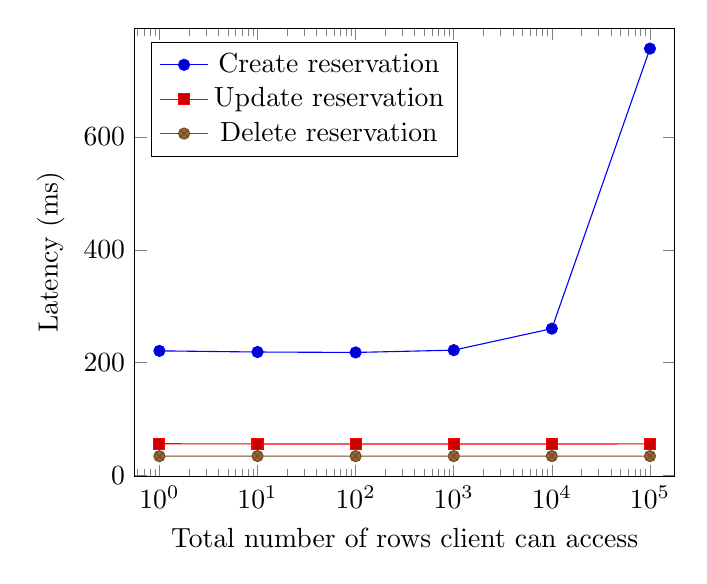
\begin{tikzpicture}
\begin{axis}[
    scaled x ticks=false,
    xticklabel style={
        /pgf/number format/fixed,
    },
    enlargelimits=0.05,
    xmode=log,
    legend pos=north west,
	ylabel=Latency (ms),
    xlabel=Total number of rows client can access,
]
\addplot coordinates {
(1,220.96589355427423)
(10,218.93483423870023)
(100,218.15750619665107)
(1000,222.23585625849358)
(10000,260.3604958467744)
(100000,756.6286911545517)
};
\addplot coordinates {
(1,56.35228721163479)
(10,56.006703622700954)
(100,56.00854317226388)
(1000,55.893261460407516)
(10000,55.839858252379386)
(100000,56.11046716505474)
};
\addplot coordinates {
(1,34.34061607207086)
(10,34.575933755274825)
(100,34.398460322658856)
(1000,34.47618348361495)
(10000,34.45739734779611)
(100000,34.448867395112416)
};
\legend{Create reservation,Update reservation,Delete reservation}
\end{axis}
\end{tikzpicture}

}

    \caption{Average latency in milliseconds for creating, updating or deleting reservations.}
    \label{fig:server-rest-mutations-latency}
\end{subfigure}
    
    \caption{Throughput for serving get, create, update and delete requests by number of rows clients may access for the REST server.}
    \label{fig:server-rest-experiment}
\end{figure}
